\section{Qu'est ce qu'un dieu dans le Proche-Orient Ancien (POA)? \\ L'exemple de Yhwh}

\begin{parag}{Noms de la région}
    \begin{itemize}
        \item Proche Orient Ancien / Ancient Near East
			\begin{itemize}
				\item Problème de l'eurocentrisme (L'orient et l'occident)
			\end{itemize}
		\item Une autre perspective: L'Asie de l'ouest
		\item Les différentes parties:
			\begin{itemize}
				\item Mésopotamie "entre les fleuves")
				\item Le Levant (Canaan) au bord de la mer
			\end{itemize}
    \end{itemize}
\end{parag}


\begin{parag}{Mésopotamie}
	Mésopotamie $\sim$ 'enre les fleuve'
	\begin{center}
	
\includegraphics[scale=0.2]{screenshots/2026-02-24.png}
	\end{center}
\end{parag}
\begin{parag}{Levan}
	\begin{center}
	
\includegraphics[scale=0.2]{screenshots/2026-02-24_1.png}
	\end{center}

\end{parag}

En general dans ce cours, on va parler de cette région:
\begin{center}

\includegraphics[scale=0.2]{screenshots/2026-02-24_2.png}
\end{center}
\subsection{Dieux}
Dans l'antiquité, on ne peut pas différencier dieux et politique, même chose pour la science.
\begin{parag}{Les noms de(s) dieu(x)}
    Voici quelque nos de participant du cours:
	\begin{itemize}
		\item Timothée
		\item  Teodora
		\item  Théophile
		\item  Théo
		\item  Samuel
		\item  Samuele
		\item  Emmanuel
		\item  Gabriel
		\item  Raphaël
		\item  Elisabeth 
	\end{itemize}
	Pour chacun de ses noms, on peut les 'retraduire' à leur équivalent avec les éléments théorophe:
	\begin{itemize}
		\item  El = Dieu
		\item  Theos = Dieu (en grec)
		\item  Abdallah
		\item  Abd al-Rahman
		\item substitution)
		\item  Jo / Jahu = Yhwh (Jonathan,
		\item eshayahu, Jean [Yochanan],
Joël) 
	\end{itemize}
	Le 'el' représente dieu, par exemple, si on prends Raphael.
	\begin{align*} \underbrace{\text{rapha}}_{= \text{soin}} + \underbrace{\text{el}}_{= \text{dieux}} \end{align*}
	
\end{parag}
\begin{parag}{Le/un dieu d'Israel: YHwh-הוהי}
	\begin{itemize}
		\item Problème/interdiction de prononcer le nom (tradition juive)
		\item le tétragramme (sans voyelles)
			\begin{itemize}
				\item Substitution du nom: Adonai (seigneur), Ha-shem (le nom)
				\item Représentation par un attribut: L'Eternel
				\item Essai de la reconstruction
				\item Facon d'écrire: YHWH, SEIGNEUR
			\end{itemize}
		\item Elohim, El = Dieu/ Divin \\
			Il qui veut aussi dire le plus grand, le Père des dieux dans la région de Levant.
			\begin{itemize}
				\item Attention pur le Levant: El est en même temps le mot pour un dieu et un dieu concret (le père des dieux)
			\end{itemize}
	\end{itemize}
	
\end{parag}
\begin{parag}{Qu'est ce qu'un dieu Levantin}
   \begin{center}
      \textbf{Les dieux agissent dans l'histoire et ont une histoire!} 
   \end{center}
   \begin{itemize}
		\item Il n'existe pas de définition fixe. Les traités théoriques sur les dieux sont plutôt des ouvrages modernes.
		\item  Dans l'Antiquité, on raconte des histoires sur les dieux et les déesses et on accomplit des rites cultuels. Mais les contenus changent sans cesse au cours de l'histoire.
		\item  La description des dieux dépend fortement du contexte et de la culture de l'époque et de la région. Des dieux disparaissent et de nouveaux apparaissent.
		\item  Les dieux eux-mêmes sont également soumis à des transformations. Dans le POA, ils changent d'avis, apprennent, modifient leur position dans le monde divin.
   \end{itemize}
   \begin{framedremark}
   Donc le titre du cours est qu'est ce qu'un dieux, neanmoins, cela est impossible, la seule représentation que nous pouvons nous faire est par les récits, pas très fiable. Notamment dire qu'un dieu n'a qu'un aspect est aussi pas très veridicte. Dans le Proche-Orient ancient, on a Mardouk qui évolue dans le temps. Dans les textes biblique on nous dit en premier lieu que la création de l'humain est parfaite, quelque temps plus tard, on revient sur notre avis.
   \end{framedremark}
   \begin{subparag}{Question}
       Est ce que Mardouk a influencé d'autre état? Une réponse ou plutot un exemple serait que par exemple, lors d'une bataille entre deux états avec des dieux différents: L'état gagnant a le dieu le plus fort.
   \end{subparag}
\end{parag}
\begin{parag}{Yhwh et l'histoire}
    Au centre de l'Ancien Testament:
	\begin{center}
	    'Non pas qui ou quoi est Dieu, mais comment il est reconnu et décrit comme agissant dans le monde, auprès de son peuple et auprès de chaque individu.'
	\end{center}
	
\end{parag}

\begin{parag}{L'iconographie -- deux exemple d'Ougarit}
    \begin{center}
    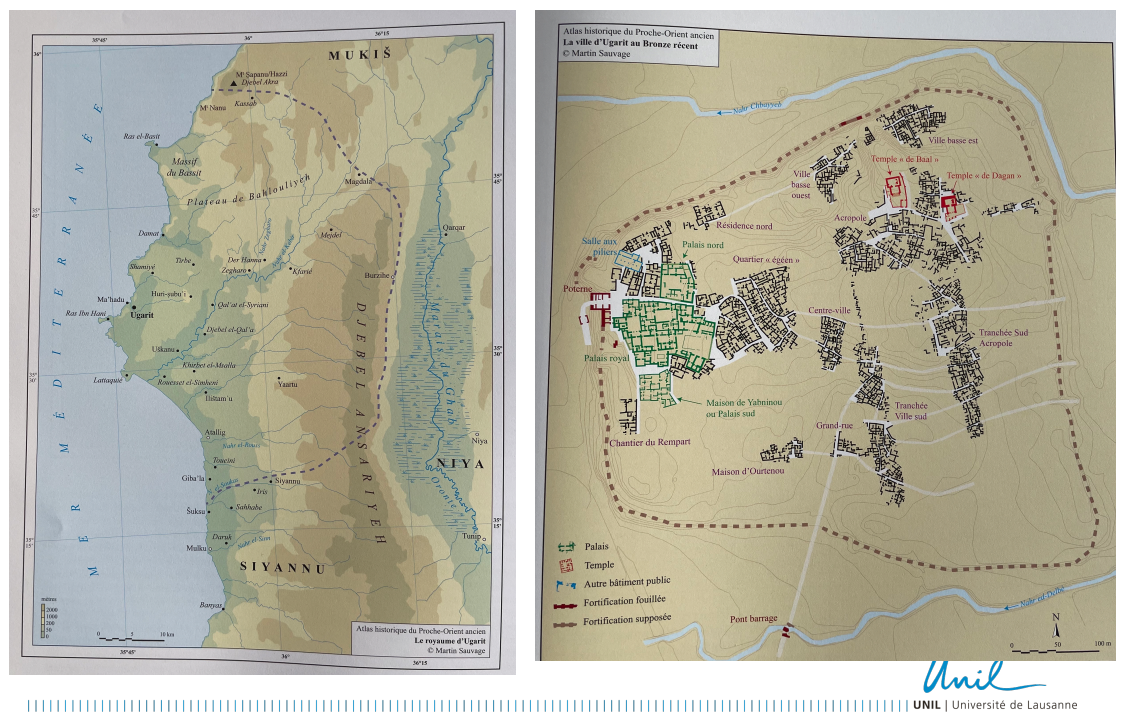
\includegraphics[scale=0.2]{screenshots/2026-02-24_3.png}
    \end{center}
	A son pique, le royaume faisait 'environ' la taille du canton de Vaud.\\

	Comme on peut voir sur l'image à droite, nous avons plusieurs temple chacun pour un dieu:
\end{parag}
\begin{parag}{Anat (ou Astarté) et Baal (15/14 a.e.c.)}
    \begin{center}
    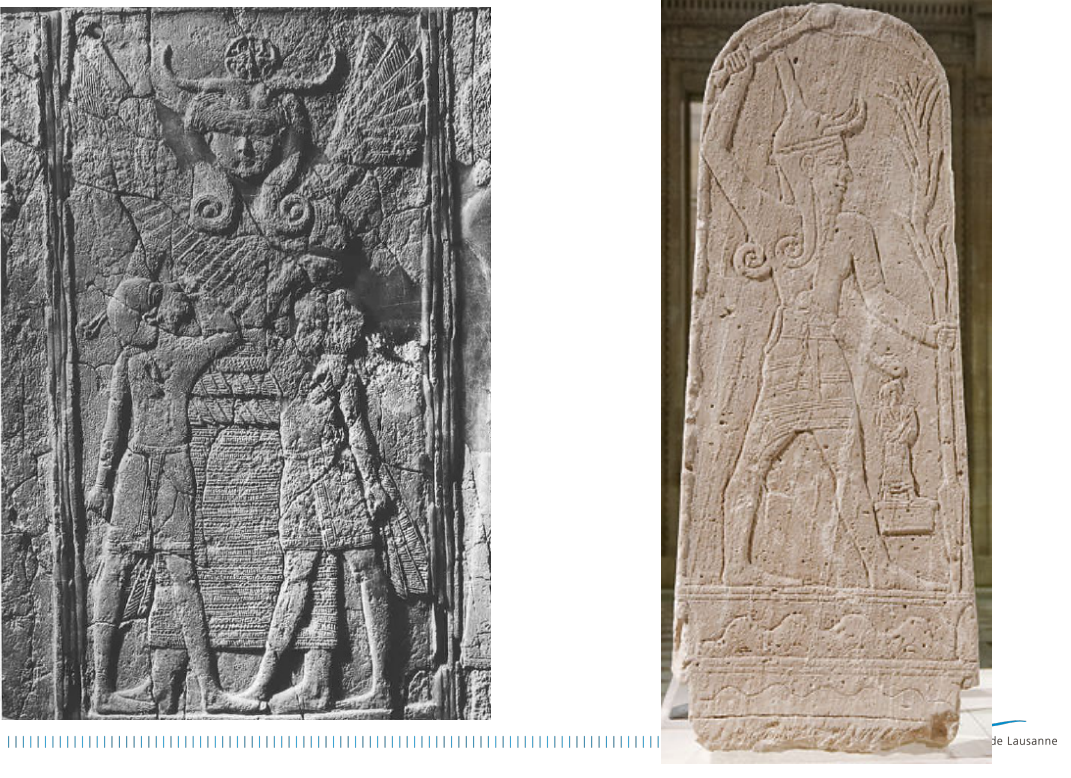
\includegraphics[scale=0.2]{screenshots/2026-02-24_4.png}
    \end{center}
	Donc ici, on a un dieu et une déesse:\\ 
	On remarque en premier que les deux dieux possèdent des cornes, les cornes sont \important{uniquement porté par les dieux}, elle représente le pouvoir.
\end{parag}
\begin{center}
\begin{minipage}{0.45\textwidth}
	A gauche, on peut voir la désse alaiter les deux humains \important{plus petit} que la déesse\\
	$ $\\
	On peut aussi voir que la déesse a des ailes, pour montrer qu'on parle d'une divinité
\end{minipage}
\hfill
\begin{minipage}{0.45\textwidth}
	Ici on a le dieux en grand et le roi en petit. Malgrès qu'il soit petit cela montre que le roi est proche de dieux.\\
	$ $\\
	Maintenant on voit qu'il y a trois bras, il possède un ...
	Important de voir que c'est aussi le dieux de la météo.
\end{minipage}
\end{center}
\begin{parag}{Les signes des divinités dans le POA}
    \begin{center}
    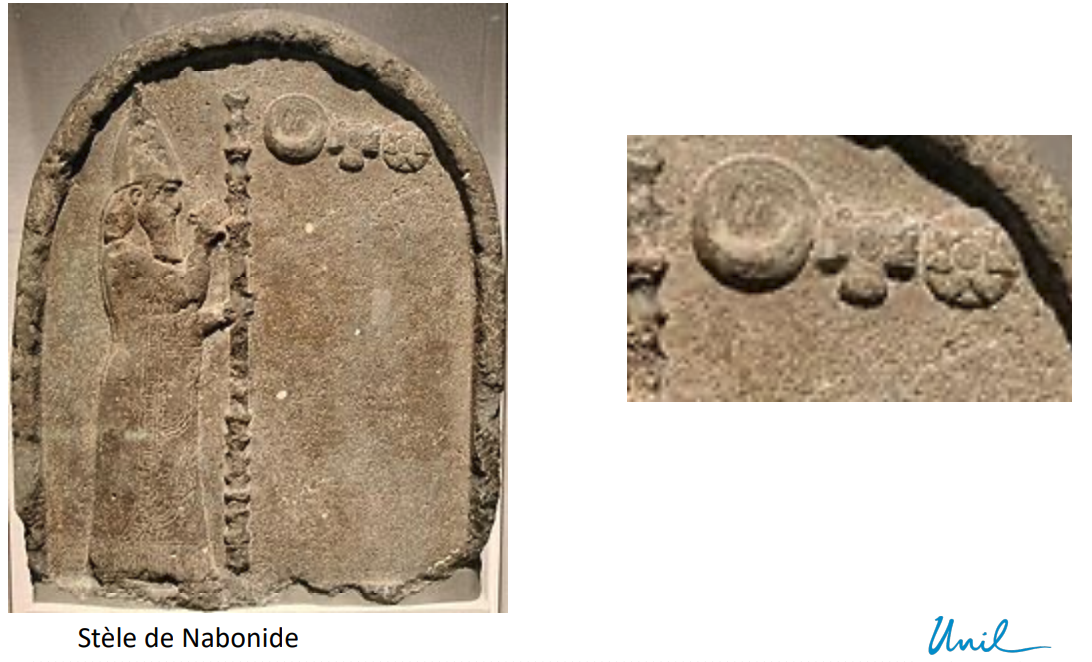
\includegraphics[scale=0.2]{screenshots/2026-02-24_5.png}
    \end{center}
	Premier truc étonnant ici et que la lune se trouvent devant le soleil, c'est le dieux de la lune.
	\begin{center}
	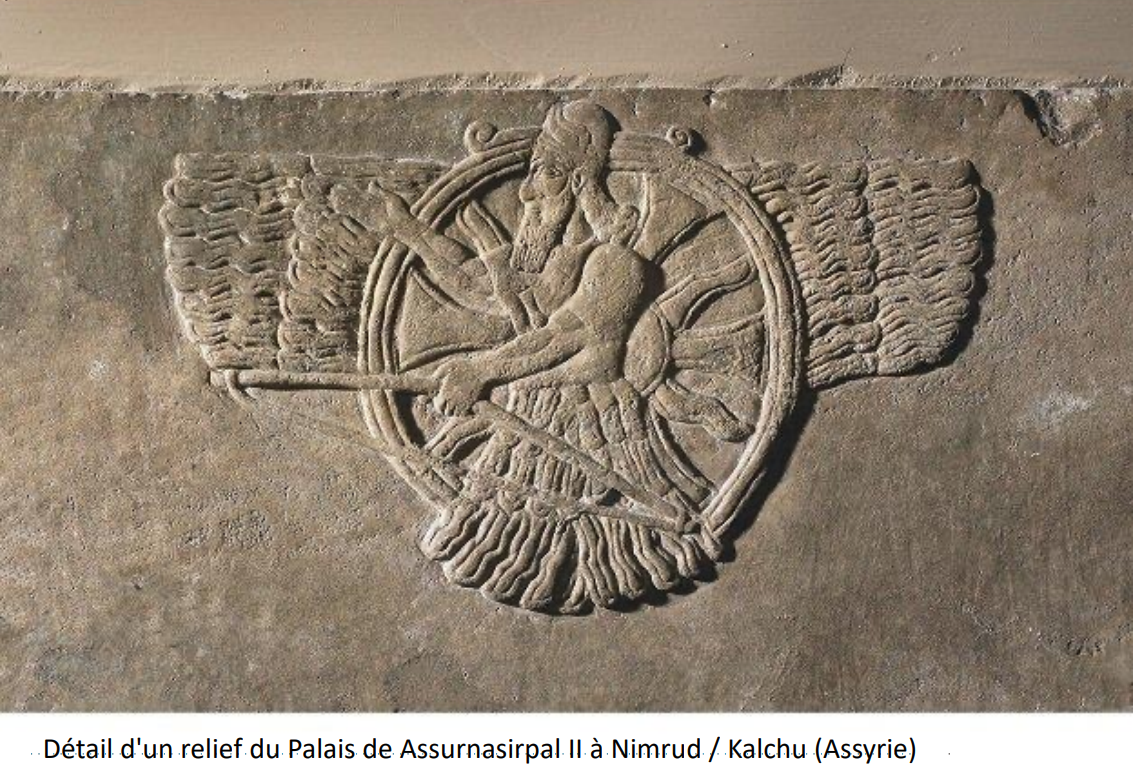
\includegraphics[scale=0.2]{screenshots/2026-02-24_6.png}
	\end{center}
	Comment vu sur les précédentes images, on a les cornes qui montre que c'est une divinité. La divinité en question est shamash le dieux du soleil aussi responsable de la guerre:\\
	$ $\\
	On a donc derrière lui le soleil, on a une combinaison de lui est le soleil. Il est armé, un arc, des armes derrière lui.
\end{parag}
\begin{parag}{Les dieux (et rois) sur les stèles}
    \begin{itemize}
        \item Objet de culte/ vénération
        \item Programme iconographique classique:
			\begin{itemize}
				\item Couronne à cornes
				\item Signes de pouvoir
				\item Les proportions sont des rapports de force
				\item En Mésopotamie: Soleil, lune et étoiles (étoile du matin ou sept étoile) pour les grands dieux, p.ex Shamash, Sin Ishtar.
			\end{itemize}
			
    \end{itemize}
    
\end{parag}



\subsection{Et en Israel}

\begin{figure}[h!]
	\centering
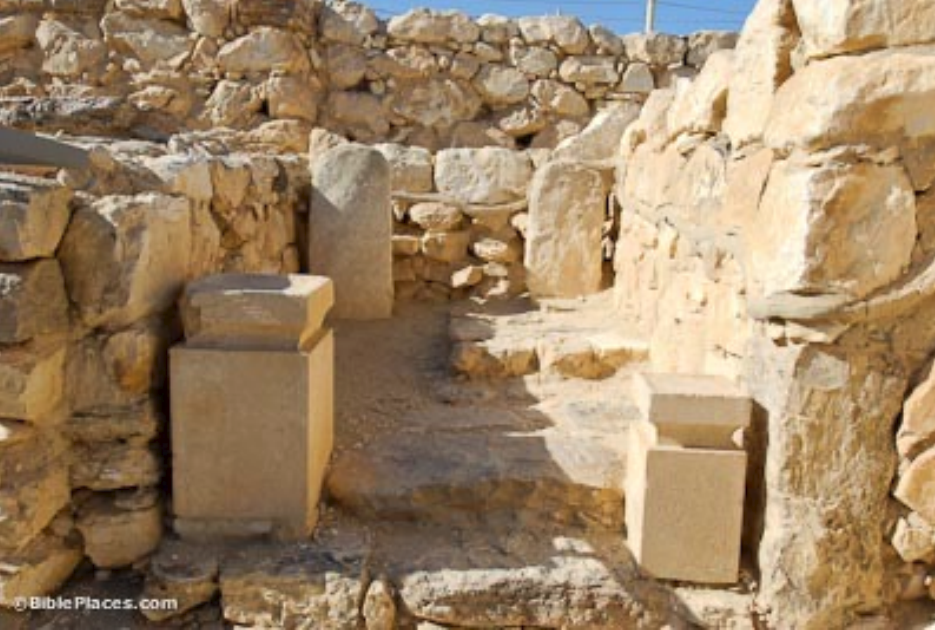
\includegraphics[scale=0.2]{screenshots/2026-02-24_7.png}
\caption{Tel Arad en Israel, temple}
\end{figure}
Donc ce que cette image montre est que l'on sait rien... On a longtemps pensé que c'etait un truc blabla, et qu'il avait une femme qui l'accompagnait (très fréquent dans la région). Néanmoins, après avoir fait la datation des pierres, on remarque que les deux pierres proviennent de date différentes, cela veut dire que nous avons eu seulement qu'une seule stèle dans ce sanctuère.
\begin{parag}{Yhwh en Israel}
    \begin{itemize}
		\item  Critique des stèles, massèbes (pierres dressées) par quelques courants théologiques en Israël ancien.
		\item  Il n'y a pas d'illustrations figuratives, mais quelques symboles, comme le soleil ailé restent et les textes de la Bible Hébraïque utilisent les mêmes images que celles qui apparaissent dans l'ensemble du POA.
    \end{itemize}
\end{parag}
\begin{parag}{Un exemple: Le soleil de Justice}
\end{parag}
\begin{center}
\begin{minipage}{0.45\textwidth}
	En \important{Mésopotamie}, Shamash est le dieu soleil. Il est aussi le dieu de la Justice
\end{minipage}
\hfill
\begin{minipage}{0.45\textwidth}
	\begin{center}
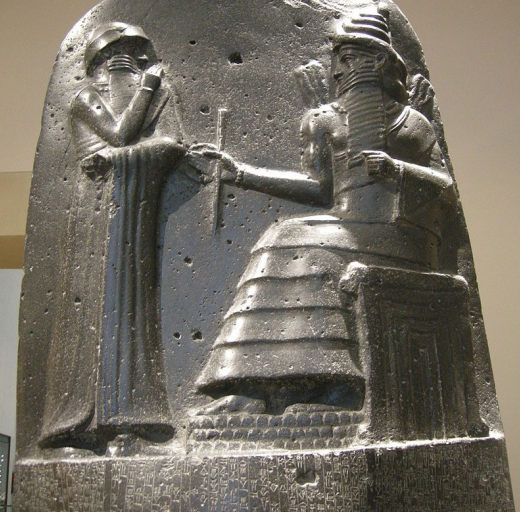
\includegraphics[scale=0.3]{screenshots/2026-02-24_8.png}

Stèle du Codex Hammurabi, Louvre
	\end{center}
	Donc on peut voir plusieurs chose, en premier lieu, la personne est assise, plus grande, avec des cornes $\implies$ divinité.
\end{minipage}
\end{center}
\begin{parag}{Ancien Testament (Malachie 3, 20-22)}
\end{parag}
\begin{center}
\begin{minipage}{0.45\textwidth}
\begin{center}
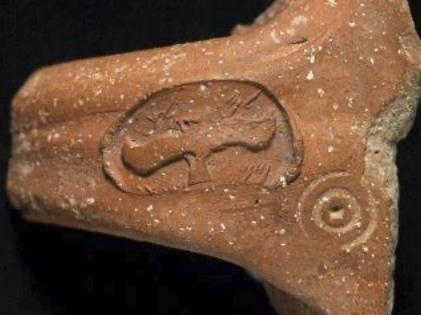
\includegraphics[scale=0.3]{screenshots/2026-02-24_9.png}

\begin{center}
    Empreint de sceau: Pour le roi 7e siècle AEC
\end{center}

\end{center}
\end{minipage}
\hfill
\begin{minipage}{0.45\textwidth}
$^{20}$Pour vous qui craignez mon nom, le \important{soleil de justice} se lèvera, portant la guérison dans ses rayons. Vous sortirez et vous gambaderez comme des veaux à l'engrais. $^{21}$Vous piétinerez les méchants, car ils seront comme cendre sous la plante de vos pieds en ce jour que je prépare, dit le Yhwh Zebaoth. $^{22}$Souvenez-vous de la Loi de Moïse, mon serviteur, à qui j'ai donné, à l'Horeb, des lois et des coutumes pour tout Israël. 
\end{minipage}
\end{center}
à partir du $^{22}$, on a ce dieu qui parle de l'histoire, c'est quelque chose de très typique (à completer).






\begin{parag}{Les autoprésentations de ce dieu}
    Dans l'exode 3,14, si on traduit:
	\begin{center}
	    Je suis qui je suis/ je suis qui je serai/ je serai qui je serai
	\end{center}
	\begin{itemize}
	    \item Jeu de mot avec le nom Yhwh et la racine hyh 'être'
	    \item En réalité, ce nom est lié au verbe hwh 'souffler' et montre que ce dieu était à l'origine un dieu de la météo (comme Baal)
	\end{itemize}
	Dans l'exode 34,6-7, si on traduit:
	\begin{center}
	    $^{6}$Et Yhwh passa devant lui [Moïse], et s’écria: Yhwh, Yhwh, Dieu miséricordieux et compatissant, lent à la colère, riche en bonté et en fidélité, $^{7}$qui conserve son amour jusqu’à mille générations, qui pardonne l’iniquité, la rébellion et le péché, mais qui ne tient point le coupable pour innocent, et qui punit l’iniquité des pères sur les enfants et sur les enfants des enfants jusqu’à la troisième et à la quatrième génération!
	\end{center}
	Meme la on peut voir que le dieu ne montre pas qu'il a une fonction, on montre plus la relation entre le dieu et l'humain
	\begin{framedremark}
	Les textes ici sont toujours écrit par des humains.
	\end{framedremark}

	Si on regarde en \important{KUNTILLET 'AJRUD'}:
	\begin{center}
	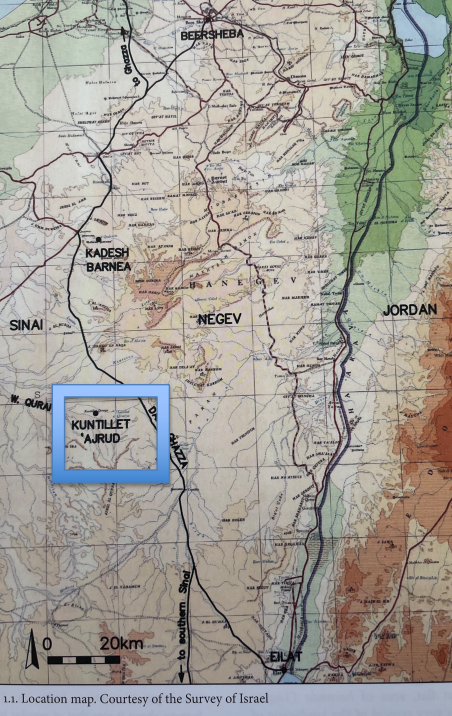
\includegraphics[scale=0.2]{screenshots/2026-02-24_10.png}
	\end{center}
	En 1975, on a fouillé un site dans la région KUNTILLET 'AJURD', ce que nous avons trouvé:
\end{parag}
\begin{center}
\begin{minipage}{0.45\textwidth}
\begin{center}
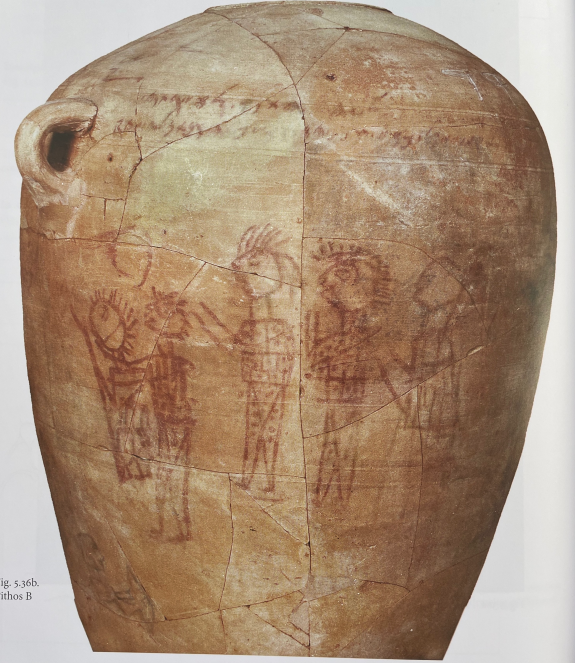
\includegraphics[scale=0.2]{screenshots/2026-02-24_11.png}
\end{center}
\end{minipage}
\hfill
\begin{minipage}{0.45\textwidth}
Message of ’Amaryāw: 
\begin{center}
“Say to my lord, are you well? I have blessed you by YHWH of Têmān and His asherah. May He bless you and may He keep you, and may He be with my lord [forever(?)”\\
\end{center}
$ $\\
On a donc on peu bien se poser la question, est ce que c'est sa femme? Alors peut-être, on ne sait pas vraimment si on a une \important{personne} ou alors une \important{force} de dieu.
\end{minipage}
\end{center}
\begin{itemize}
	\item Il n'y a pas de panthéon (développé) en Israël et la monolâtrie et le monothéisme se développent de plus en plus.
\end{itemize}
\important{Néanmoins}:
\begin{itemize}
	\item  D'autres êtres divins restent actifs dans le monde céleste et souterrain.
	\item  Cela ne signifie toutefois pas qu'il n'y ait jamais eu de culte d'autres divinités. Mais le Dieu unique réunit de plus en plus en lui les aspects d'autres divinités.
\end{itemize}

Néanmoins, cela veut aussi dire que des \important{déesses} étaient vénérées, mais leur domaines faisaient également de plus en plus partie de la divinité unique.\\
$ $\\
Dieu n'est donc pas défini par son genre (il ait p. ex. comme mère et père).



\begin{parag}{Déportation des statues divines (Nimrud)}
    \begin{center}
    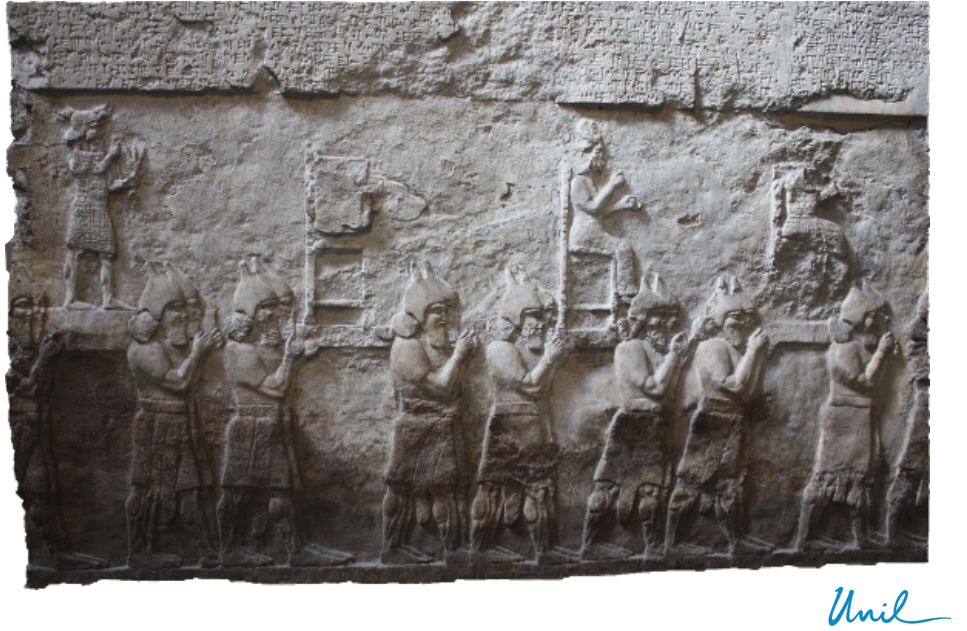
\includegraphics[scale=0.2]{screenshots/2026-02-24_12.png}
    \end{center}
	Esaie 44,13-20 (TOB (traduction)):
	\begin{center}
	   "L'artisan sur bois tend le cordeau, trace l'œuvre à la craie, l'exécute au ciseau, oui, la trace au compas, lui donne la tournure d'un homme, la splendeur d'un être humain, pour qu'elle habite un temple, pour qu'on débite des cèdres en son honneur. On prend du rouvre et du chêne, pour soi on les veut robustes, parmi les arbres de la forêt, on plante un pin, mais c'est la pluie qui le fait grandir. C'est pour l'homme bois à brûler : il en prend et se chauffe, il l'enflamme et cuit du pain."
	\end{center}
	
	Donc on vient de créer une statue de boie par un arbre planté par un humain \important{mais} a grandit grace à dieu (pluie) cette statue est utilisé pour faire une représentation d'une divinité.\\
	$ $\\
	La suite:
	\begin{center}
	   "Avec ça il réalise aussi un dieu et il se prosterne, il en fait une idole et il s'incline devant elle. Il en fait flamber la moitié dans le feu et met par-dessus la viande qu'il va manger : il fait rôtir son rôti et se rassasie ; il se chauffe aussi et dit : « Ah, ah, je me chauffe, je vois le rougeoiement ! » Avec le reste il fait un dieu, son idole, il s'incline et se prosterne devant elle, il lui adresse sa prière, en disant : « Délivre-moi, car mon dieu, c'est toi ! » Ils ne comprennent pas, ils ne discernent pas, car leurs yeux sont encrassés, au point de ne plus voir, leurs cœurs le sont aussi, au point de ne plus saisir ! Nul en son cœur ne fait retour à la compréhension et au discernement, de manière à dire : « J'en ai fait flamber la moitié dans le feu, j'ai aussi cuit du pain sur les braises, je rôtis de la viande et je la mange, et du surplus, je ferais une abjection, je m'inclinerais devant un bout de bois ! » Il s'attache à de la cendre, son cœur abusé l'égare : il ne se verra pas délivré ! Il ne dira pas pour autant : « N'est-ce pas tromperie, ce que j'ai en main ? »"
	\end{center}
	Pourquoi le double usage du bois ici est un problème?
	\begin{itemize}
		\item Il veut être délivré en parlant avec un bout de bois. un bout de bois qui pourrait être utilisé pour se chauffer. On voit que le texte est un peu sarcastique, 'il essaie de faire un truc qu'on sait qui ne sert a rien ce looser'
	\end{itemize}
	
\end{parag}
\begin{parag}{Deutéronome 4,27-28}
    Dieu parle avec Israel et annoce l'exil en Baylonie:
	\begin{center}
	   « Yhwh vous dispersera parmi les peuples, et il ne restera de vous qu'un petit nombre parmi les nations, là où Yhwh vous aura emmenés. Là-bas, vous servirez des dieux qui sont l'ouvrage de la main des hommes : du bois, de la pierre, incapables de voir et d'entendre, de manger et de sentir. » 
	\end{center}
	Donc si on a un dieu qui ne peut pas manger, on a un dieu qui ne peut rien faire et donc qui ne sait à rien.
\end{parag}

\subsubsection{Problème des idoles}
\begin{itemize}
	\item Esaie 40-55: Critique de l'idolatrie
	\item Idolatrie: Vénération des idoles
		\begin{itemize}
			\item Les idoles/images ne sont pas le problème, mais la pratique cultuelle
		\end{itemize}
	\item Il s'agit d'une polémique, une diffamation et non d'une dscription neutre des pratiques!
\end{itemize}
On a un autre culte et on se \important{moque} du culte des autres.


\begin{parag}{Le Dieu de l'Exode}
    Deutéronome 4,19-20
	\begin{center}
" Ne lève pas les yeux vers le ciel, regarde le soleil, la lune et les étoiles, toute l'armée des cieux, et te laisse entraîner à te prosterner devant eux et à les servir ; ils ont été faits par Yhwh ton Dieu pour tous les peuples qui sont partout sous le ciel ; mais vous, Yhwh vous a pris et il vous a fait sortir de l'Egypte, cette fournaise à fondre le fer, pour que vous deveniez son peuple, son patrimoine, comme vous l'êtes aujourd'hui."
	\end{center}
	Donc on a un dieu qui a \important{crée} soleil, étoile, lune, on a un dieu qui a \important{crée} les autres dieux $\implies$ notre dieu est plus important que le votre, on a même un dieu qui communique avec les humains: pas besoin de me vénerer avec (à completer).
\end{parag}


\subsection{Qu'est ce qu'un Dieu}
\begin{center}
    \textbf{Un dieu est un dieu, quand il sait et peut communiquer et agir!}
\end{center}
\begin{parag}{Yhwh, le dieu d'Israel}
    \begin{itemize}
        \item Est le dieu de l'Exode, de la libération d'Egype
			\begin{itemize}
				\item histoire commune (idéalisée) entre dieu et peuple, l'histoire de salut
			\end{itemize}
		\item absorbe de plus en plus d'attributs d'autres divinités (météo, création, justice, processus de solarisation), et, au fil de l'histoire religieuse, devient responsable d'un nombre croissant de domaines. Du point de vue d'Israël, ses domaines de compétence s'élargissent également, il devient responsable du monde entier (universalisation) ainsi que du monde des vivant·es et des mort·es.
    \end{itemize}
    On a aussi dans l'israel ancien que le dieu ne s'occupait seulement des êtres vivants. Il n'est pas responsable du monde sous-terrain, mais a la fin de (j'ai pas la date), on a des textes qui montre qu'il commence à s'occuper d'eux à cette époque.
\end{parag}




